\documentclass{article}
\usepackage[utf8]{inputenc}
\usepackage{geometry}
\usepackage{graphicx}
\usepackage{pgfplots}
\usepackage{verbatim}
\usepackage{amssymb}
\usepackage{amsmath}
\usepackage{tcolorbox} %needed
\usepackage{comment}
\usepackage{physics}
\usepackage{mathrsfs}
\newcommand{\ints}{\displaystyle \int}
\newcommand{\lims}{\lim_{\norm{J}\rightarrow 0}\sum_{J \in P}}
\newcommand{\limn}{\lim_{n \rightarrow \infty}}
\newcommand{\sumn}{\sum_{i=1}^n}
\newcommand{\limr}{\lim_{\norm{J}\rightarrow 0}\sum_{J \in P} f(a+Ji)J \quad : \quad J=\dfrac{b-a}{n} \quad f(a + Ji)=}
\newcommand{\na}{\eta(n)}
\tcbuselibrary{listingsutf8}


\geometry{a4paper, left=2cm, right=2cm, top=1cm, bottom=2cm}

\pgfplotsset{compat=1.18}
\begin{document}

\begin{minipage}{0.7\textwidth}
    \small \textbf{GEOMETRÍA ANALÍTICA II}  \\
    \small {Facultad de Ciencias, Universidad Nacional Autónoma de México} \\
    \small {Profesora: Rocio del Pilar Aguilar Benítez} \\
    \small {Evaluado por: Ulisses Jesús Gutiérrez Hérnandez}\\
    \small {Fecha de entrega: 23 de Abril de 2024} \\
    \small {Integrantes: Andrés López González} \\
    \small {Iván Galeana Aguilar} \\
\end{minipage}
\hfill
\begin{minipage}{0.12\textwidth}
    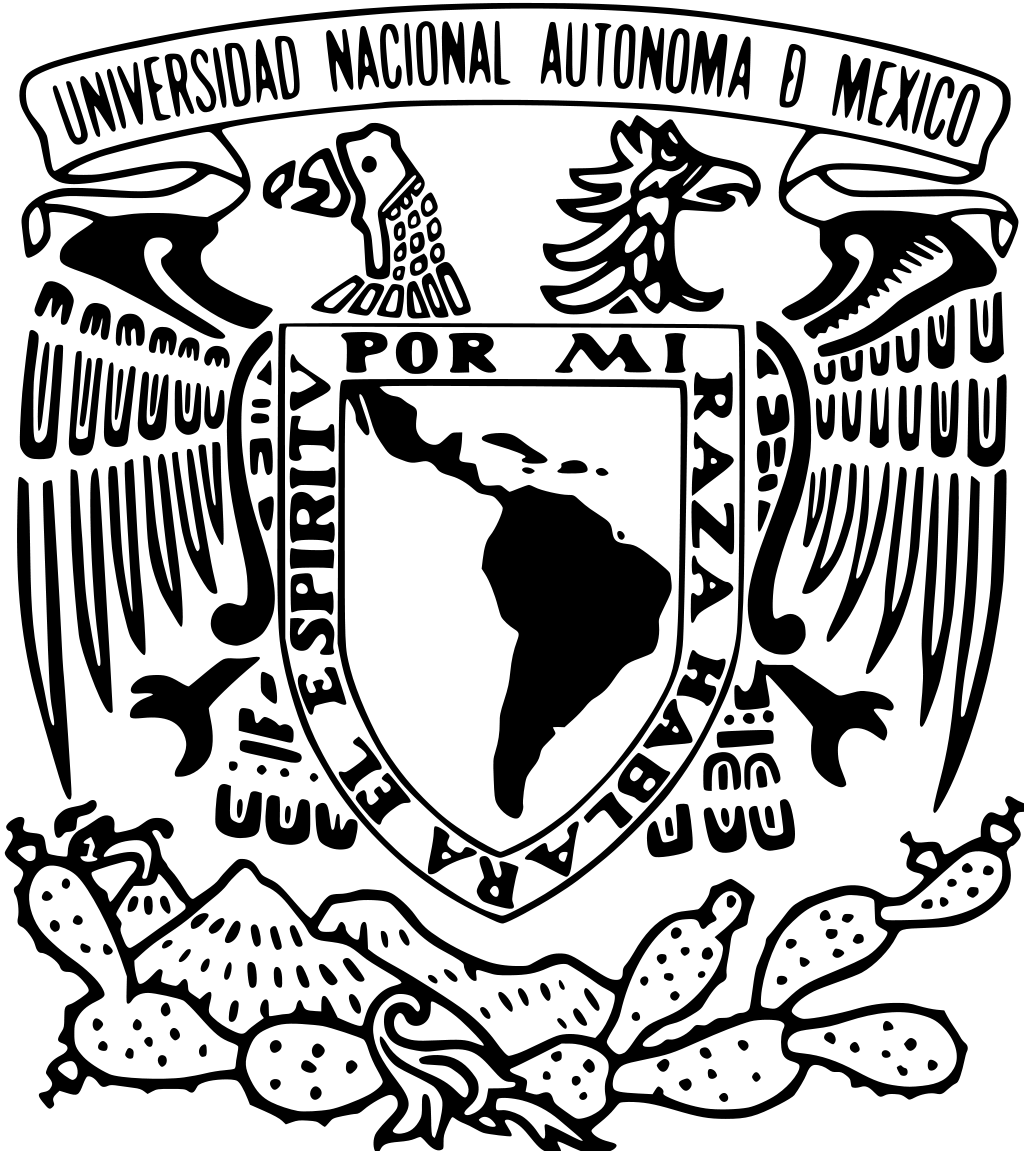
\includegraphics[width=\linewidth]{logo_universidad}
\end{minipage}

\section*{Tarea Examen II}
\noindent I. Hallar la parametrización de la superficie que se obtiene al rotar la curva
\begin{equation}
    z = \frac{\sin 3x}{2}
\end{equation}
Alrededor del eje x.\\
\textit{Nótese en Figure I. que la ecuación original es sinusoidal por lo que al no tener restricciones se alarga en forma de lámina indefinidamente a lo largo del eje y.}
\begin{figure}[h]
    \centering
    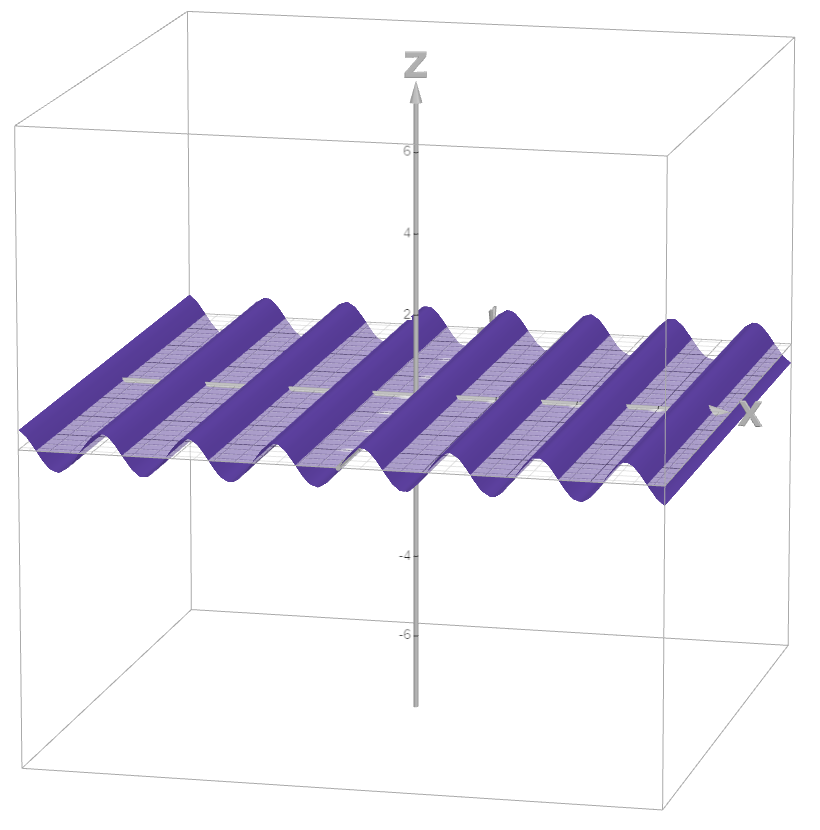
\includegraphics[width=0.75\linewidth]{Sinusoidal.png}
    \caption{Ecuación I.}
    \label{fig:enter-label}
\end{figure}\\
\textit{Para hacerlo rotar a lo largo del eje x construimos un círculo que oscile manteniendo su radio en función de x, mientras que sus dimensiones de apertura se hayan en el plano yz, es así que construimos el siguiente círculo de radio Equation. I}\\
\begin{equation}
    y^2 + z^2 = \left( \frac{\sin 3x}{2} \right)^2
\end{equation}

\newpage
Véase en Figure II. cómo se comporta perfectamente bien como pide el enunciado esta ecuación cartesiana.\\
\begin{figure}[h]
    \centering
    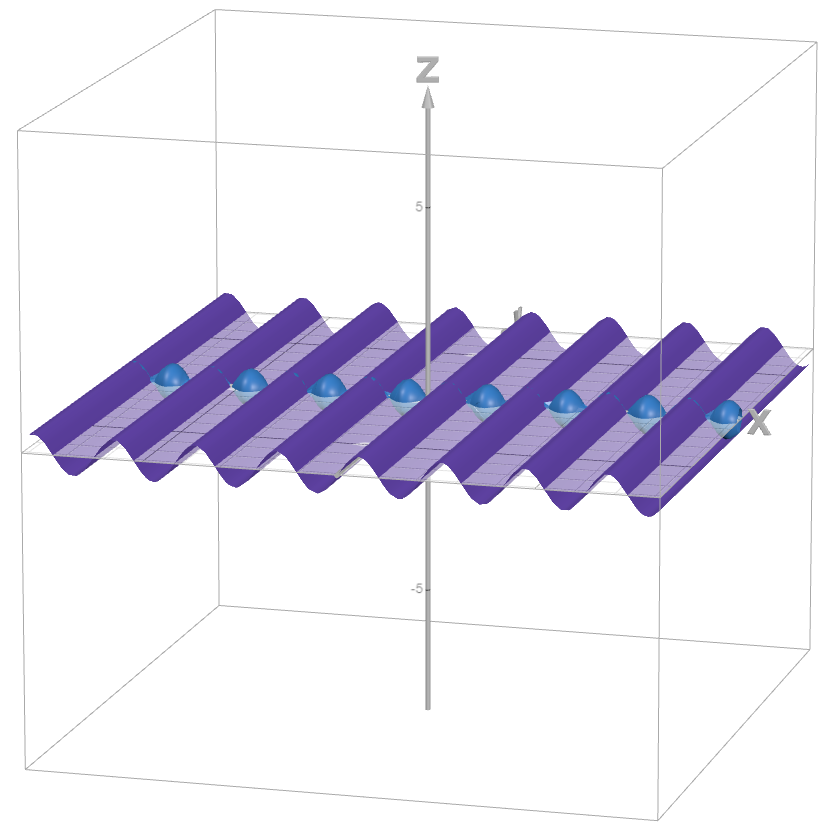
\includegraphics[width=0.70\linewidth]{Sinusoidal+Rev.png}
    \caption{Superficie resultante comparada con Ecuación I.}
    \label{fig:enter-label}
\end{figure}\\
$\therefore$ El inciso b) ha sido completado. \\
Para la parametrización es igualmente demasiado simple, construimos nuestra función que traza un círculo en yz.
\begin{equation*}
    C(s) = (0,\sin s,\cos s) \, : \, s \in [0,2\pi)
\end{equation*}
Paralelamente parametrizamos la Ecuación I.
\begin{equation*}
    S(t) = (t,0,\frac{\sin 3t}{2}) \, : \, t \in \mathbb{R}
\end{equation*}
Solo sumamos ambas parametrizaciones y está resuelto, la gráfica es exactamente la misma que Figure II por lo que no es muy relevante volverla a ver.
\begin{equation}
    \delta(s,t) = \left(t,\sin s,\frac{\sin3t}{2}+\cos s\right) \, : s\in [0,2\pi), \, t \in \mathbb{R}
\end{equation}
\begin{figure}[h]
    \centering
    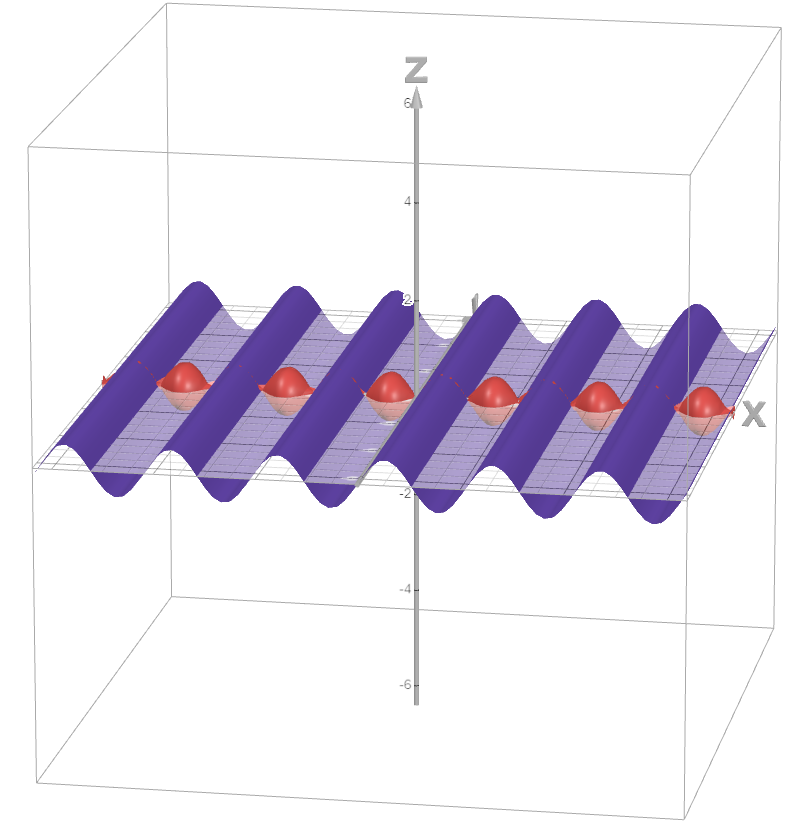
\includegraphics[width=0.25\linewidth]{Eq III.png}
    \caption{Parametrización.}
    \label{fig:enter-label}
\end{figure}
\newpage
\noindent I. Demuestre que dos planos dados por las ecuaciones \\
\begin{equation*}
    a_1x + b_1y + c_1z + d_1 = 0
\end{equation*}
\begin{equation*}
    a_2x + b_2y + c_2z + d_2 = 0
\end{equation*}
Son paralelos distintos sii $\exists k \in \mathbb{R}$ tal que $a_2=ka_1$, $b_2=kb_1$, $c_2=kc_1$ y $d_2 \neq kd_1$ \\\\
$\Rightarrow)$ Supóngase que el primer plano así como el segundo son paralelos distintos entre sí, esto quiere decir que el vector normal de ambos planos es colineal. Por construcción la magnitud de este vector normal no tiene ningún sentido geométrico pues es fácilmente alterable sin dejar rastros evidentes en la ecuación por lo cual tenemos que $\Vec{n_1}||\Vec{n_2}$.
\textit{i.e.} Alguno de ellos es una combinación lineal del otro $\Vec{n_1}=\lambda\Vec{n_2} \, \Rightarrow \, \Vec{n_1} = (a_1,b_1,c_1) = (\lambda a_1,\lambda b_1,\lambda c_1) = \lambda\Vec{n_2}$. Tal que lambda es cualquier escalar del campo y para esta demostración da igual si lo llamamos así o si se denomina k, es así que tenemos la siguiente caracterización de los planos
\begin{equation*}
    a_1x + b_1y + c_1z + d_1 = 0
\end{equation*}
\begin{equation*}
    \lambda a_1x + \lambda b_1y + \lambda c_1z + d_2 = 0
\end{equation*}
Nótese que si $d_1=\lambda d_2$ entonces al dividir toda la ecuación por $\lambda$ tendremos que las ecuaciones son exactamente la misma y por ende los planos son exactamente el mismo, que contradeciría nuestra hipótesis que son paralelos distintos, por lo que solo nos queda decir que $d_1 \neq \lambda d_2$ lo que caracterizaría el mismo plano pero en cualquier otro punto del espacio que no atraviesa al otro, por lo que queda demostrada la implicación de ida. \\
$\Leftarrow)$ Supóngase que tenemos dos planos representados de la siguiente forma:
\begin{equation*}
    a_1x + b_1y + c_1z + d_1 = 0
\end{equation*}
\begin{equation*}
    a_2x + b_2y + c_2z + d_2 = 0
\end{equation*}
De modo que $\exists k \in \mathbb{R}$ tal que $a_2=ka_1$, $b_2=kb_1$, $c_2=kc_1$ y $d_2 \neq kd_1$. Análogo que en la ida al sustituir obtenemos los siguientes planos:
\begin{equation*}
    a_1x + b_1y + c_1z + d_1 = 0
\end{equation*}
\begin{equation*}
    k a_1x + k b_1y + k c_1z + d_2 = 0
\end{equation*}
De aquí obtenemos que sus vectores normales son una combinación lineal del otro tal que $\Vec{n_1}=k\Vec{n_2}$, por lo que para todo punto $\Vec{p}$ perteneciente al plano, existirá un punto en el otro plano que al ser multiplicado por $k$ se tendrá el punto $\Vec{p}$; por otro lado se definió por hipótesis que $d_2 \neq kd_1$, por lo que el punto al que se desplazó el plano será distinto para ambos para todo punto de este, por lo cual esto y la naturaleza de los vectores normales colineales jamás se tocarán (a menos que nos pongamos Euclideanos y consideremos la recta extendida unión el infinito o espacios surrealistas, pero creo que no es el caso). \\
$\therefore$ La proposición ha sido demostrada.

\newpage
\noindent III. Eliminar el término mixto en la ecuación de la curva y dibujarla.
\begin{equation}
    2xz - x^2 + z^2 + 3 = 0
\end{equation}
Representamos los términos en su forma matricial $A \in M_3(\mathbb{R})$ : $A(\Vec{x}) = 2xz - x^2 + z^2$. Este paso es algoritmizable con la fórmula presentada en clase así que directamente sustraeremos $\lambda \textbf{I}$ para obtener los subespacios invariantes, primero utilizando el tensor alternante "determinante" de $\textbf{A} - \lambda \textbf{I}$ igualado a cero obtendremos los eigenvalores como se vió en clase. El método a usar será el determinante por menores.
\begin{equation*}
    det\begin{vmatrix}
        -1-\lambda & 0 & 1 \\
        0 & -\lambda & 0 \\
        1 & 0 & 1-\lambda
    \end{vmatrix} = -(1+\lambda)(-\lambda)(1-\lambda)-1(1)(-\lambda) = \lambda(1^2-\lambda^2)+\lambda = 2\lambda - \lambda^3 = 0
\end{equation*}
Esto nos resulta en una ecuación igualada a cero de un polinomio de tercer orden, vease que es casi directa la resolución:
\begin{align*}
    2\lambda - \lambda^3 &= 0 \\
    \Rightarrow \lambda_1 = 0 \\
    2\lambda - \lambda^3 &= 0 \\
    2 - \lambda^2 &= 0 \\
    2 &= \lambda^2 \\
    \pm \sqrt{2} &= \lambda_{2,3}
\end{align*}
Necesitamos ahora obtener los eigenvectores, este proceso por la naturaleza de nuestra matriz es el más tedioso; primero igualamos $(\textbf{A} - \lambda \textbf{I})(\Vec{x})$ al origen $\Vec{0}$ para conseguir un sistema de ecuaciones 3x3.
\begin{equation}
    \begin{bmatrix}
        -1-\lambda & 0 & 1 \\
        0 & -\lambda & 0 \\
        1 & 0 & 1-\lambda
    \end{bmatrix}
    \begin{pmatrix}
        x \\ y \\ z
    \end{pmatrix} = 
    \begin{pmatrix}
        -x(1+\lambda)+z \\
        -\lambda y \\
        x + (1-\lambda)z
    \end{pmatrix} =
    \begin{pmatrix}
        0 \\ 0 \\ 0
    \end{pmatrix} \quad \forall \lambda_i \in eigenvector_A
\end{equation}
Veamos que si $\lambda=0$ entonces tenemos $z-x=0$, $0y = 0$ y $x+z=0$, esto solo nos deja la posibilidad que tanto x como z sean cero, dado que queremos una base ortonormal en la aplicación lineal es conveniente fijar a y (que como no aparece en el sistema es independiente) como uno. Es así que nuestro primer eigenvector sea.
\begin{equation*}
    T(\hat{e_1}) = (0,1,0)
\end{equation*}
Nótese que de hecho para cualquier valor de lambda en $\mathbb{R}$ y es un término que no depende de x,z así que reducimos el sistema para los siguientes eigenvectores.
\begin{equation*}
    \begin{pmatrix}
        -x(1+\lambda)+z \\
        x + (1-\lambda)z
    \end{pmatrix} =
    \begin{pmatrix}
        0 \\ 0
    \end{pmatrix} \quad \forall \lambda_i \in eigenvector_A
\end{equation*}
Considérese en este caso $\lambda=\sqrt{2}$, en algún momento llegaremos a una tautología de 0=0 para todo valor de x,z así que lo mejor es expresar a x en términos de z. Usaremos la segunda fila.
\begin{equation*}
    x = (\sqrt{2}-1)z
\end{equation*}
i.e. Nuestro eigenvector para x=1 es...
\begin{equation*}
    T(\hat{e_2}) = \frac{(1, 0, \sqrt{2}-1)}{\norm{\Vec{\lambda_2}}} = \frac{(1, 0, \sqrt{2}-1)}{\sqrt{1+2-2\sqrt{2}+1}} = \left( \frac{1}{\sqrt{4-2\sqrt{2}}}, 0, \frac{\sqrt{2}-1}{\sqrt{4-2\sqrt{2}}}\right)
\end{equation*}
Con un método análogo obtenemos que con la primera fila y $\lambda=-\sqrt{2}$.
\begin{equation*}
    x=(\sqrt{2}+1)z
\end{equation*}
i.e. Nuestro eigenvector para x=1 es...
\begin{equation*}
    T(\hat{e_3}) = \frac{(1, 0, \sqrt{2}+1)}{\norm{\Vec{\lambda_3}}} = \frac{(1, 0, \sqrt{2}+1)}{\sqrt{4+2\sqrt{2}}} = \left(\frac{1}{\sqrt{4+2\sqrt{2}}},0,\frac{\sqrt{2}+1}{\sqrt{4+2\sqrt{2}}}\right)
\end{equation*}

 \newpage
 Ya que tenemos nuestros eigenvectores existe un teorema que toda aplicación lineal puede ser representada por una matriz y cualquier cambio en su ordenamiento provoca permutación en la orientación de sus ejes, como es visualmente probable que la rotación se haya hecho intencionalmente en el eje x,z entonces representaremos la siguiente transformación lineal isomorfa de columnas ortonormales que manda generadores linealmente independientes en generadores linealmente independientes bajo el siguiente orden.
 \begin{equation*}
     (x,y,z) =
     \begin{bmatrix}
         \dfrac{1}{\sqrt{4+2\sqrt{2}}} & 0 & \dfrac{1}{\sqrt{4-2\sqrt{2}}} \\
         0 & 1 & 0 \\
         \dfrac{\sqrt{2}+1}{\sqrt{4+2\sqrt{2}}} & 0 & \dfrac{\sqrt{2}-1}{\sqrt{4-2\sqrt{2}}}
     \end{bmatrix}
     \begin{pmatrix}
         x' \\ y' \\ z'
     \end{pmatrix}
     = \left(\dfrac{1}{\sqrt{4+2\sqrt{2}}}x' + \dfrac{1}{\sqrt{4-2\sqrt{2}}}z',1,\dfrac{\sqrt{2}+1}{\sqrt{4+2\sqrt{2}}}x' + \dfrac{\sqrt{2}-1}{\sqrt{4-2\sqrt{2}}}z' \right)
 \end{equation*}
Sustituyendo se tiene...

$2[(\frac{1}{\sqrt{4+2\sqrt{2}}}x' + \frac{1}{\sqrt{4-2\sqrt{2}}}z'][\frac{\sqrt{2}+1}{\sqrt{4+2\sqrt{2}}}x' + \frac{\sqrt{2}-1}{\sqrt{4-2\sqrt{2}}}z'] - [\frac{1}{\sqrt{4+2\sqrt{2}}}x' + \frac{1}{\sqrt{4-2\sqrt{2}}}z']^2 + [\frac{\sqrt{2}-1}{\sqrt{4-2\sqrt{2}}}z']^2 + 3 = 0$

 
\begin{figure}[h]
    \centering
    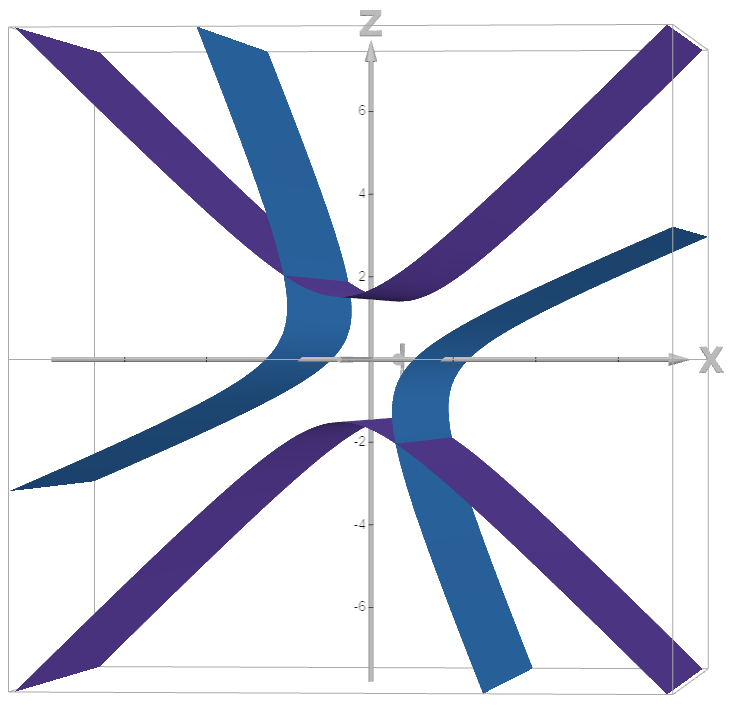
\includegraphics[width=0.75\linewidth]{EcRotación.png}
    \caption{Ecuación sin término cruzado}
    \label{fig:enter-label}
\end{figure}\\
\begin{figure}[h]
    \centering
    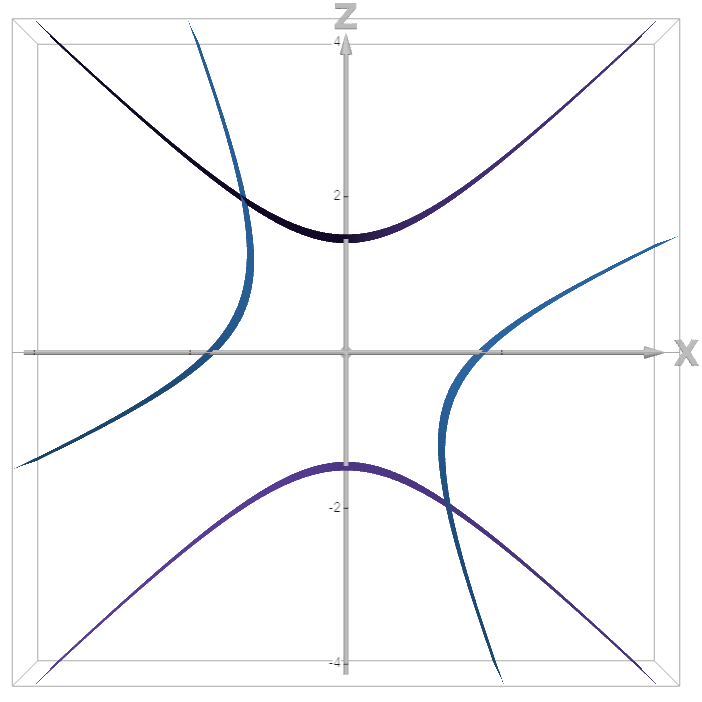
\includegraphics[width=0.25\linewidth]{Frontal.png}
    \caption{Vista frontal}
    \label{fig:enter-label}
\end{figure}

\newpage
V. Hallar la parametrización de la superficie reglada T(S(M)) donde M se obtiene pegando la recta
\begin{equation}
    \mathscr{L}: (x,y,z)=t(2,1,-1) \, : \, t \in \mathbb{R}
\end{equation}
A lo largo de la curva
\begin{equation}
    \mathscr{C}: z = -2y^2 \quad x=0
\end{equation}
En donde.
\begin{equation}
S(\Vec{x}) =
\begin{bmatrix}
1 & 0 & 0\\
0 & \frac{1}{\sqrt{2}} & -\frac{1}{\sqrt{2}}\\
0 & \frac{1}{\sqrt{2}} & \frac{1}{\sqrt{2}}
\end{bmatrix} 
\begin{pmatrix}
x\\y\\z
\end{pmatrix} \end{equation}
\begin{equation}
 T(\Vec{x}) = \Vec{x} + (4,2,10)   
\end{equation}
La ecuación M es simplemente la suma de las parametrizaciones $\mathscr{L}$ y $\mathscr{C}$, quienes son bastante triviales de realizar por lo que no se profundizará en ello.
\begin{equation}
    \Vec{\mathscr{L}} + \Vec{\mathscr{C}} = M = (2t, t+s, -t -2s^2) \, : \, t,s \in \mathbb{R}
\end{equation}
\begin{figure}[h]
    \centering
    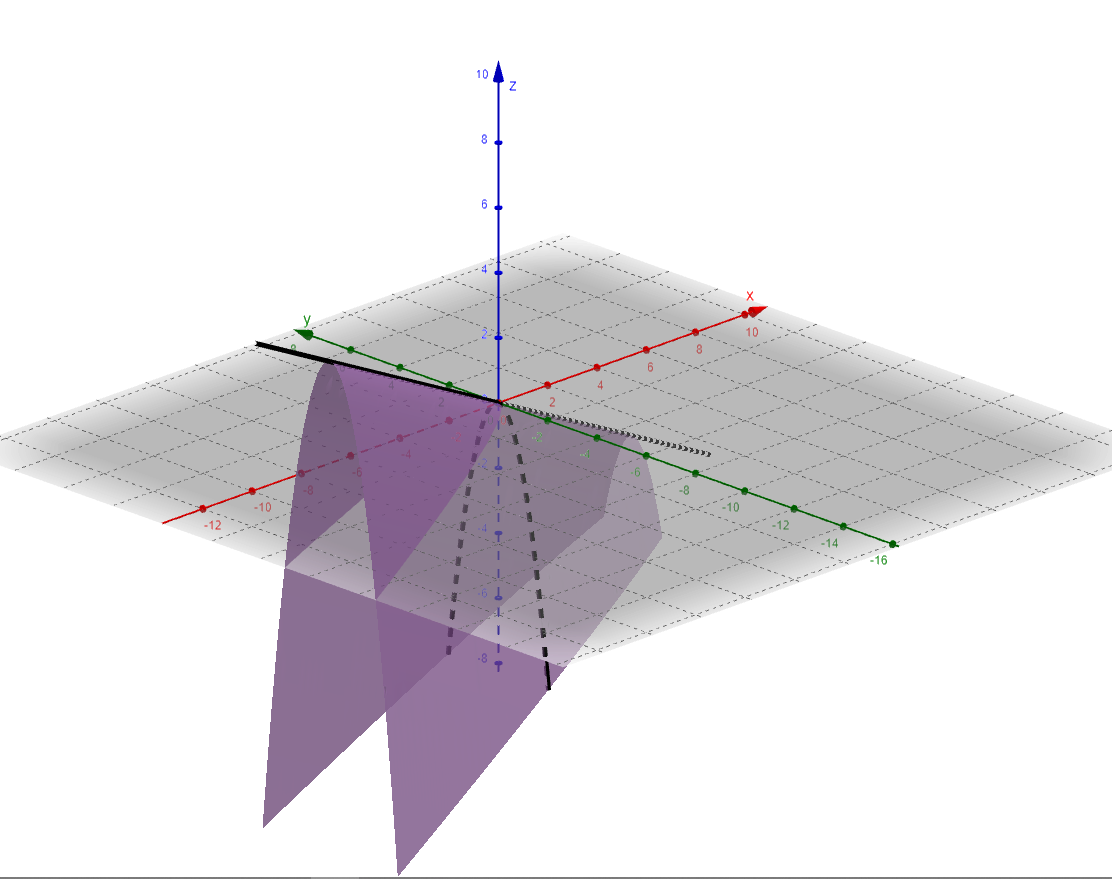
\includegraphics[width=0.75\linewidth]{M.png}
    \caption{Gráfica de M}
    \label{fig:enter-label}
\end{figure}\\
Ahora solo obtenemos T(S(M))
\begin{equation}
T(S(M)) = S(M) + (4,2,10) = \begin{bmatrix}
1 & 0 & 0\\
0 & \frac{1}{\sqrt{2}} & -\frac{1}{\sqrt{2}}\\
0 & \frac{1}{\sqrt{2}} & \frac{1}{\sqrt{2}}
\end{bmatrix} 
\begin{pmatrix}
2t\\t+s\\-t - 2s^2
\end{pmatrix} + (4,2,10) \end{equation}
Haciendo el producto matricial finalmente tenemos
\begin{equation}
    \left(2t, \frac{2s^2+s+2t}{\sqrt{2}}, \frac{-2s^2+s}{\sqrt{2}}\right) + (4,2,10) = \left(2t + 4, \frac{2s^2+s+2t+2\sqrt{2}}{\sqrt{2}}, \frac{-2s^2+s+10\sqrt{10}}{\sqrt{2}}\right)
\end{equation}
\newpage
\begin{figure}[h]
    \centering
    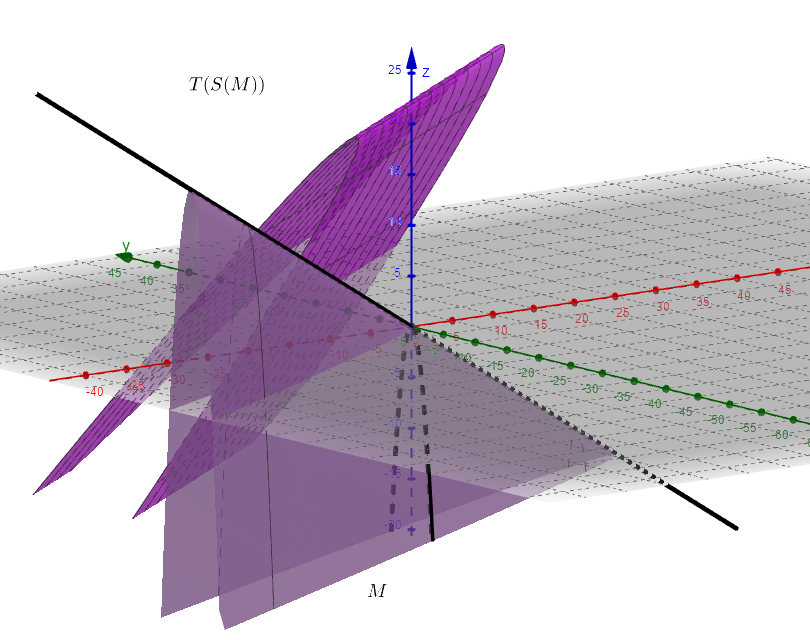
\includegraphics[width=0.75\linewidth]{T(S(M)).png}
    \caption{Composición de transformaciones}
    \label{fig:enter-label}
\end{figure}

\newpage
III. (2) Obtenga, en cada uno de los siguientes incisos, una ecuación cartesiana que describa el lugar geométrico dado por la ecuación polar correspondiente\\
\textit{Considérese lo siguiente}
\begin{equation}
    x^2+y^2=r^2
\end{equation}
\begin{equation}
    x = r\cos\vartheta
\end{equation}
\begin{equation}
    y= r\sin\vartheta    
\end{equation}


\noindent a) $r=4$\\
Por Equation XII.
\begin{equation*}
    x^2+y^2=4^2
\end{equation*}


\noindent b) $r=4\sin \vartheta$\\
Por el cociente de Equation XIII y Equation XIV
\begin{equation*}
    \arctan \frac{y}{x} = \vartheta
\end{equation*}
De Equation XII deducimos
\begin{equation*}
    x^2+y^2=4^2\sin^2 \left(\arctan \frac{y}{x}\right)
\end{equation*}
c) $r = \frac{5}{\sin \vartheta - \cos \vartheta}$ \\
La ecuación es directa pero haré explícita el álgebra usada, consideremos Eq XIII y Eq XIV.
\begin{align*}
    r\sin \vartheta - r\cos \vartheta &= 5 \\
    y - x &= 5 \\
    x + 5 &= y
\end{align*}
d) $r = \frac{4}{4+\sin\vartheta}$ \\
Considérese trivial por Eq. XIV: $\sin^2\vartheta = \frac{y^2}{r^2} = \frac{y^2}{x^2 + y^2}$.
\begin{align*}
    r^2 = \frac{4^2}{4^2 + 8\sin\vartheta + \sin^2\vartheta} &= x^2 + y^2 \\
    \frac{4^2}{4^2 + 8\frac{y}{\sqrt{x^2+y^2}} + \frac{y^2}{x^2+y^2}} &= x^2 + y^2 \\
    (x^2 + y^2)(16 + 8\frac{y}{\sqrt{x^2+y^2}} + \frac{y^2}{x^2+y^2}) &= 4^2 \\
    \textit{Fuertemente simplificado...}& \\
    16x^2+17y^2+8y\sqrt{x^2+y^2} &= 4^2
\end{align*}
\textit{Todos los reactivos han sido verificados en Desmos.}

\end{document}



\end{document}